\svnid{$Id: rt_general.tex 1 2015-08-30 15:39:28Z rodriqu_dd $}

\chapter{Projecten, schermen en schermindeling}
\label{ch:general}

In dit hoofdstuk wordt een overzicht gegeven van de algemene functionaliteit van Ringtoets. Na een korte introductie wordt in dit hoofdstuk allereerst aandacht besteed aan de projectstructuur die door RT wordt gebruikt. Vervolgens worden de hoofdfuncties van de gebruikersinterface uitgelegd voor alle type beschikbare vensters. Als laatste wordt aandacht besteed aan de mogelijkheden tot importeren en exporteren van data en resultaten.

\section{Project structuur}
	\label{sec:RT_Project_Structure}
RT werkt met een projectstructuur die weergegeven wordt in het \textbf{Project} toolvenster (zie paragraaf \ref{sec:RT_Project_Explorer}). Data en modellen kunnen aan het project worden toegevoegd op de volgende manieren:

\begin{enumerate}
	\item Klik op \textbf{New Folder}, \textbf{New Item} of \textbf{New Model} in de \textbf{Home} tab bovenaan het scherm, zoals weergegeven in figuur \ref{fig:rt_Add_Object}.
	\item Rechtsklik in het \textbf{Project} toolvenster op de gewenste locatie en klik dan op \textbf{New Item...} of \textbf{New Folder}, zoals weergegeven in figuur \ref{fig:rt_Add_Object_Project_Explorer}.
\end{enumerate}

\begin{figure}[H]
	\centering
		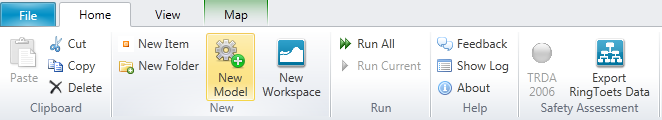
\includegraphics[width=1.0\textwidth]{figures/chapter_general/Home_Ribbon_Add_New_Model.png}
		\caption{Voorbeeld van de Home tab met daarin onder het kopje Add de mogelijkheid tot het toevoegen van een object aan het project.}
	\label{fig:rt_Add_Object}
\end{figure}
\begin{figure}[H]
	\centering
		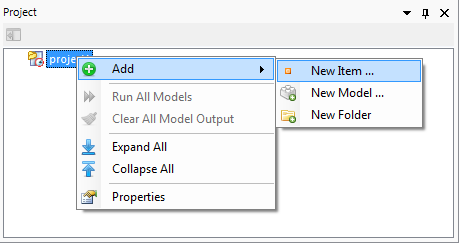
\includegraphics{figures/chapter_general/rt_Add_Object_Project_Explorer.png}
		\caption{Voorbeeld van het context menu dat naar voren komt bij rechts klikken op het project. Door op Add te klikken krijgt de gebruiker de mogelijkheid objecten aan het project toe te voegen.}
	\label{fig:rt_Add_Object_Project_Explorer}
\end{figure}

De objecten in een RT project zijn doorgaans afgeleid van een van de drie soorten zoals hieronder weergegeven (en nader omschreven):
\begin{itemize}
\item \textbf{Item} - Geeft data weer van een willekeurig type
\item \textbf{Model} - Geeft een model weer
\item \textbf{Folder} - Geeft een folder weer vergelijkbaar met een directory in het windows besturingssysteem
\end{itemize}

\subsection{Item}
Een item kan willekeurige informatie bevatten. RT kent drie type items die altijd aanwezig zijn:
\begin{itemize}
\item Map (World) - Voegt een lege kaart toe aan het project
\item Text Document - Voegt een leeg tekst document toe aan het project
\item Web link - Voegt een weblink toe aan het project
\end{itemize}
Naast een item is er doorgaans ook een (document) venster beschikbaar om de inhoud van het item te bekijken en zo mogelijk aan te passen. In dat geval is het venster te openen door dubbel te klikken op het desbetreffende item in het \textbf{Project} toolvenster of via een klik met de rechter muisknop op het item in het project toolvenster en dan op \textit{Open}.

\subsection{Model}
Een model is een rekenkern met bijbehorende invoer en uitvoer. Standaard heeft een model in DeltaShell dus ook een folder \textit{Input} en een folder \textit{Output}. In de input en output folders is er plaats voor items die de invoer en uitvoer beschrijven. Het laten rekenen van een model kan op verschillende manieren:
\begin{itemize}
\item Rechtsklik op het model in het \textbf{Project} toolvenster en dan klik op \textbf{Run Model}
\item Klik op 
\includegraphics{figures/chapter_general/Run_Arrow.png} (run) of 
\includegraphics{figures/chapter_general/RunAll_Arrow.png} (run All) in de \textbf{Home} tab van de ribbon (zie ook paragraaf \ref{sec:RT_Toolbar})
\item Selecteer een model en druk op F9, of druk op Ctrl+F9 om alle modellen in het project te laten rekenen
\end{itemize}

\subsection{Folder}
Een Folder in een RT project is vergelijkbaar met een map, folder of directory in het windows bestandssysteem. Een map kan worden gebruikt om gegevens (items en modellen) te ordenen en groeperen. Folders worden ook gebruikt in Modellen om input items en output items te groeperen.

\section{Interface onderdelen}
	\label{sec:DS:InterfaceOnderdelen}
Figuur \ref{fig:RT_Welcome_Page} geeft een overzicht van de interface, waarbij zoveel mogelijk schermen zichtbaar zijn gemaakt. Deze paragraaf bespreekt de aangegeven onderdelen. De gebruikersinterface is georganiseerd in een set van tool- en documentvensters. Deze kunnen naar wens worden gerangschikt en gepositioneerd in de interface. Daarnaast heeft de interface een quick access toolbar (1 in de figur) en ribbon (2 in de figuur) om het project, de data of de weergave te kunnen sturen of bewerken. Deze paragraaf geeft allereerst aandacht aan de mogelijkheden die de gebruiker heeft om het gebruik van de interface zo goed mogelijk aan te laten sluiten bij zijn eigen wensen. Daarna zullen alle toolvensters en document vensters kort worden toegelicht. Nummers in de beschrijving refereren naar de nummers in figuur \ref{fig:RT_Welcome_Page}.

\subsection*{Toolvensters}
Toolvensters geven de eigenschappen van het huidig geselecteerde item weer. In RT zijn de volgende toolvensters beschikbaar:
\begin{itemize}
\item Project (3)
\item Map (4)
\item Chart (5)
\item Properties (6)
\item Messages (7)
\end{itemize}

\begin{figure}[H]
	\centering
		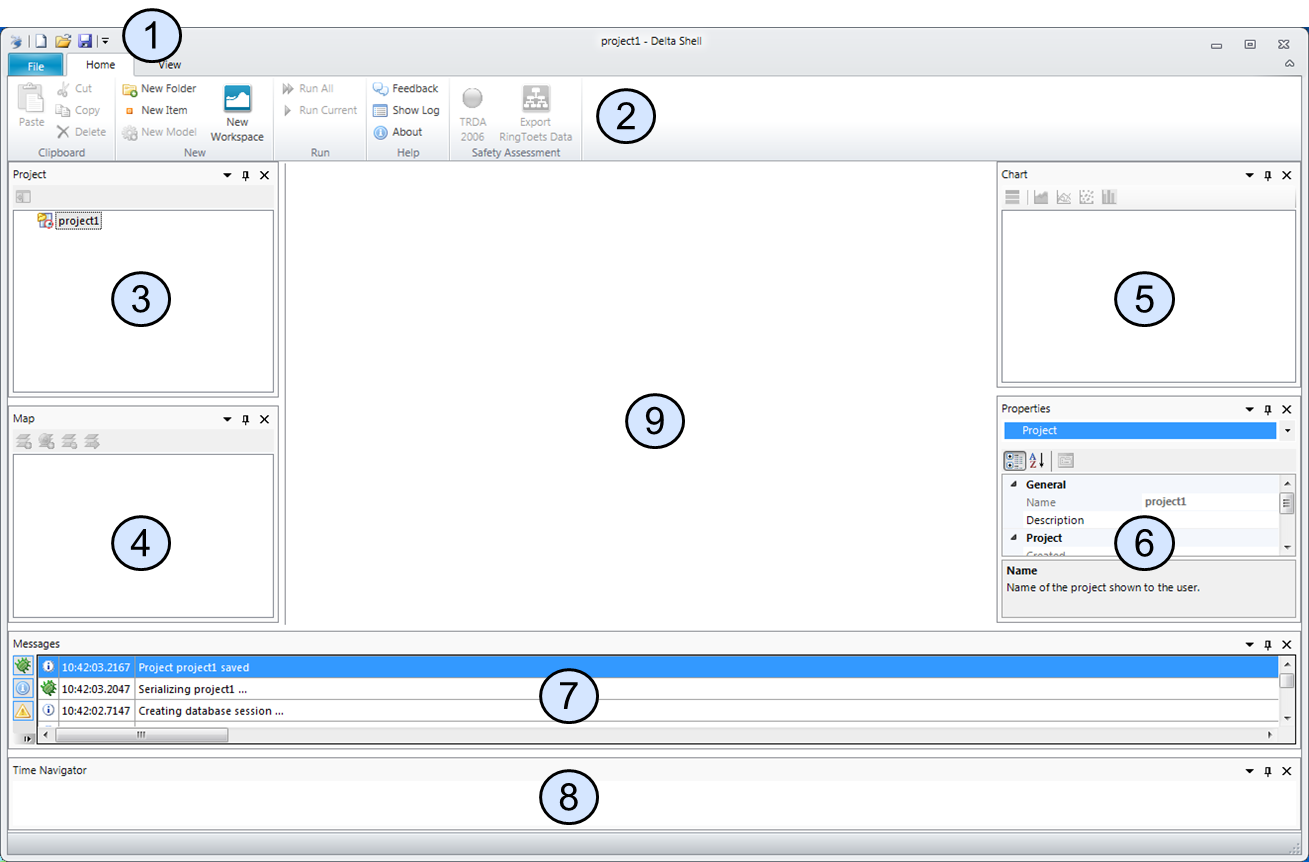
\includegraphics[width=\textwidth]{figures/chapter_general/rt_Welcome.png}
		\caption{De RT interface}
	\label{fig:RT_Welcome_Page}
\end{figure}


\subsection*{Document vensters}
Document vensters worden gebruikt voor het visualiseren en het bewerken van specifieke gegevenstypen. Ze worden geopend in het hoofdvenster (9) dat centraal staat na het opstarten van RT. Voorbeelden van document vensters zijn:
\begin{itemize}
\item Map(s)
\item Editors
\item Visualizers
\end{itemize}


\subsection{Hoofdvenster}
Het hoofdscherm is de plek waar alle documentvensters die door de gebruiker zijn geopend (bijvoorbeeld kaarten en editors) bekeken en bewerkt kunnen worden. Het venster beschikt over een tabstructuur vergelijkbaar met tabs in een Excel document. De gebruiker kan door middel van de pijltjes rechtsboven door de tabs navigeren. Docking en het verplaatsen van vensters (zie paragraaf \ref{sec:RT_Docking}) maakt het mogelijk om op een overzichtelijke manier verschillende document vensters naast elkaar te gebruiken.

\subsection{Docking en aanpassen van vensters}
\label{sec:RT_Docking}
De grafische gebruikersinterface kan eenvoudig aangepast worden aan persoonlijke voorkeuren door docking van vensters. Dit is mogelijk door een venster met de linker muisknop te slepen en los te laten links, rechts, boven of onder door middel van een hulpwijzer (zie figuur \ref{fig:3_Docking}). Dit kan gedaan worden met alle geopende tabs, maar ook met toolvensters. Er kan ook worden gekozen om een venster los van het hoofdscherm weer te geven (Floating). Wanneer een venster geopend is bevinden zich rechtsboven twee symbolen (zie ook figuur \ref{fig:3_Pin_UnPin}), waarmee:
\begin{itemize}
\item het venster op het scherm vastgezet kan worden of naar een tab verplaatst kan worden (de punaise)
\item het venster van het scherm verwijderd wordt en via de menubalk weer opgeroepen kan worden (het kruisje)
\end{itemize}

Ook de grootte van de vensters is geheel naar eigen wens aan te passen door met de muis op de lichtgekleurde grens tussen twee vensters te gaan staan en vervolgens met de linker muisknop ingedrukt de grootte van een venster aan te passen.

\begin{figure}[H]
	\centering
		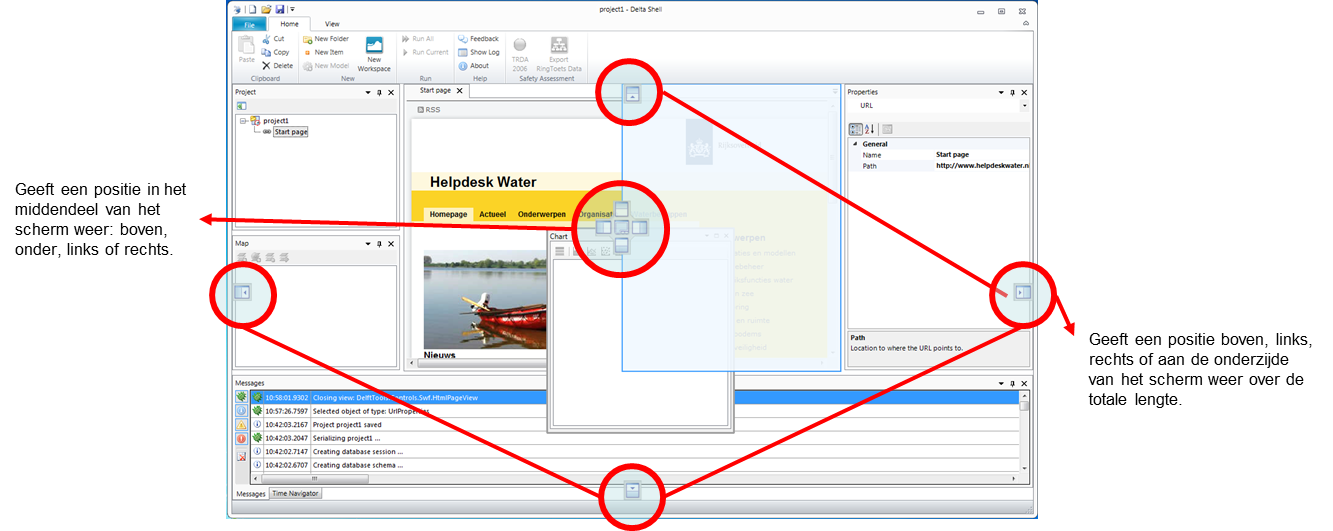
\includegraphics[width=\textwidth]{figures/chapter_general/rt_Docking_explained.png}
		\caption{Voorbeeld van de hulpwijzer voor docking van een toolvenster}
	\label{fig:3_Docking}
\end{figure}

\begin{figure}[H]
	\centering
		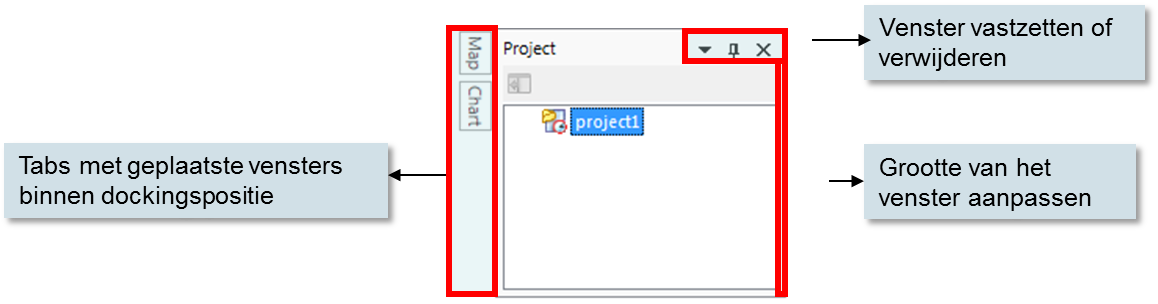
\includegraphics[width=\textwidth]{figures/chapter_general/rt_Pin_UnPin_Explained.png}
		\caption{Uitleg van de mogelijkheden voor het vastzetten, verbergen of vergroten/verkleinen van een venster}
	\label{fig:3_Pin_UnPin}
\end{figure}

\subsection{Ribbon}
	\label{sec:RT_Toolbar}
Aan de bovenkant van de interface bevindt zich een zogenaamed ribbon bar (nummer 2 in figuur \ref{fig:RT_Welcome_Page}). In de ribbon bieden knoppen functionaliteit aan voor bijvoorbeeld het gebruik in een document venster (zoals een kaart), of voor het doen van bewerkingen in het project (snelfuncties). De ribbon bar heeft verschillende tabs:

\begin{itemize}
	\item[Home] Dit is een algemene tab waar veel handige knoppen beschikbaar zijn die kunnen worden gebruikt bij het werken met een project (figuur \ref{fig:rt_Ribbon_Home})
	\item[View] Deze tab biedt de mogelijkheid om toolvensters weer zichtbaar te maken indien ze bijvoorbeeld door een klik op het kruisje zijn weggehaald (figuur \ref{fig:RT_Ribbon_View})
	\item[Chart] De Chart tab geeft de mogelijkheid tot het exporteren of aanpassen van de lettergrootte wanneer een grafiek zichtbaar is in een van de documentvensters (figuur \ref{fig:rt_Ribbon_Chart})
	\item[Map] Met behulp van deze tab kan een kaart worden aangepast aan de wensen van de gebruiker wanneer deze zichtbaar is in een van de documentvensters (figuur \ref{fig:RT_Ribbon_Map})
\end{itemize}

\begin{figure}[H]
	\centering
		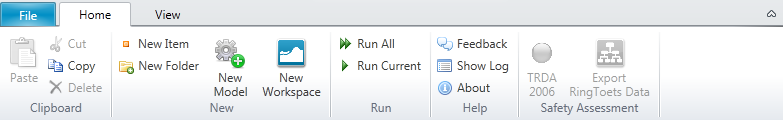
\includegraphics[width=1.0\textwidth]{figures/chapter_general/rt_Home.png}
		\caption{Overzicht van de beschikbare functies in de Home ribbon tab}
	\label{fig:rt_Ribbon_Home}
\end{figure}

\begin{figure}[H]
	\centering
		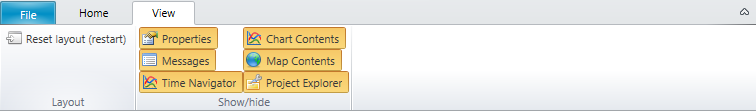
\includegraphics[width=1.0\textwidth]{figures/chapter_general/rt_View.png}
		\caption{Overzicht van de beschikbare functies in de View ribbon tab}
	\label{fig:RT_Ribbon_View}
\end{figure}

\begin{figure}[H]
	\centering
		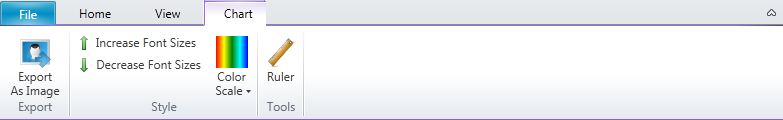
\includegraphics[width=1.0\textwidth]{figures/chapter_general/rt_Chart.png}
		\caption{Overzicht van de beschikbare functies in de Chart ribbon tab}
	\label{fig:rt_Ribbon_Chart}
\end{figure}

\begin{figure}[H]
	\centering
		\includegraphics[width=1.0\textwidth]{figures/chapter_general/RT_Map.png}
		\caption{Overzicht van de beschikbare functies in de Map ribbon tab}
	\label{fig:RT_Ribbon_Map}
\end{figure}

\subsection{Project}
	\label{sec:RT_Project_Explorer}
Het \textbf{Project} toolvenster is het belangrijkste venster voor de navigatie door projectgegevens. In dit toolvenster zijn alle project componenten te zien in een boomstructuur (zie figuur \ref{fig:RT_Project_Explorer}). Binnen het venster kan het project geordend worden door het toevoegen van Folders (zie paragraaf \ref{sec:RT_Project_Structure}) en het slepen van items, of het gebruik van cut (Ctrl+X) en paste (Ctrl+V). Het project toolvenster kan worden verborgen of verwijderd, door gebruik te maken van de punaise of het kruisje rechts bovenaan (zie ook paragraaf \ref{sec:RT_Docking}). Na verwijdering kan het venster worden opgehaald door een muisklik op het de \textbf{Project} button in de \textbf{View} ribbon tab (zie ook figuur \ref{fig:RT_Ribbon_View}). Door te klikken op het pictogram linksboven in het project toolvenster wordt het actieve item in het hoofdvenster gelokaliseerd in de boomstructuur van het Project toolvenster.

\begin{figure}[H]
	\centering
		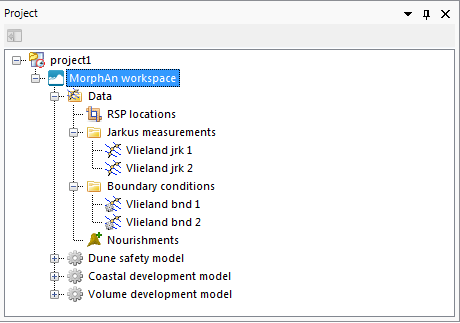
\includegraphics{figures/chapter_general/Project_Explorer_RTData.png}
		\caption{Voorbeeld van het Project toolvenster met een veel voorkomende RT project structuur}
	\label{fig:RT_Project_Explorer}
\end{figure}

Er bestaan verschillende mogelijkheden om de project structuur te bekijken of bewerken:
\begin{itemize}
\item linker muisklik om te selecteren
\item rechter muisklik geeft een menu met beschikbare acties
\item dubbelklik om document venster te tonen, afhankelijk van het item of model waarop geklikt is
\end{itemize}

\subsection{Map}
	\label{sec:RT_MapView}
RT biedt de mogelijkheid om een GIS kaart te bewerken. 

% TODO: Describe all buttons in the Map ribbon

Het is mogelijk om een standaard achtergrondkaart in te stellen die wordt gebruikt overal waar een kaartlaag wordt getoond (zie paragraaf \ref{sec:RT_Map_Contents}). Dit kan de gebruiker doen door een nieuwe kaart toe te voegen aan het project (of een bestaande kaart op te zoeken in het \textbf{Project} toolvenster) en via het rechter muis menu (context menu) te kiezen voor "`Use as default background layer"'. Vervolgens wordt de kaart in het toolvenster dik gedrukt en wordt deze als achtergrondkaart toegevoegd overal waar een kaart wordt weergegeven. Het is ook mogelijk een standaard achtergrondkaart aan te maken via de setup wizard voor een RT workspace.

\begin{figure}[H]
	\centering
		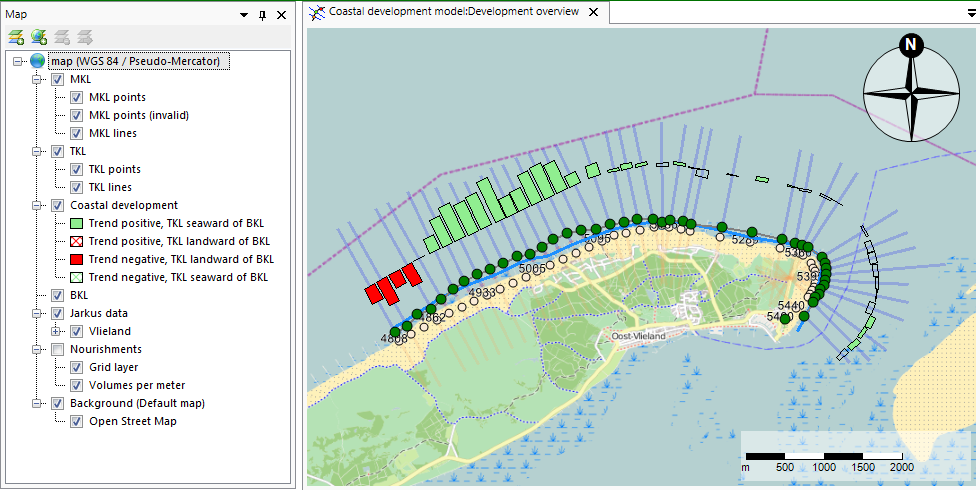
\includegraphics[width=0.85\textwidth]{figures/chapter_general/Map_With_MapContents.png}
		\caption{Voorbeeld van een kaart met resultaten van het Coastal Development Model}
	\label{fig:RT_Map}
\end{figure}

\subsection{Map toolvenster}
	\label{sec:RT_Map_Contents}
Indien een kaart (Map) actief is in het document venster (figuur \ref{fig:RT_Map}), kunnen de kaartlagen worden beheerd in het toolvenster \textbf{Map} (figuur \ref{fig:Map_Contents}).

Met de vier pictogrammen linksboven in het map toolvenster kunnen nieuwe lagen worden toegevoegd of verwijderd op basis van bijvoorbeeld shapefiles (.shp) of TIFF bestanden (.tiff) met georeference. Daarnaast is het mogelijk om een laag op de kaart te exporteren naar een shapefile. Met de knoppen rechtsboven kan het venster worden verwijderd of verborgen. Het venster kan worden opgehaald door te klikken op menu item \textbf{Map} in de \textbf{View} ribbon (zie ook figuur \ref{fig:RT_Ribbon_View}).

Elke laag kan (on)zichtbaar gemaakt worden door het te selecteren of deselecteren. Dit kan gedaan worden voor een laag als geheel, maar ook voor sublagen binnen een laag (indien deze sublagen bevat). Door te dubbelklikken op een laag, wordt de laag properties editor geopend met daarin symbolen, maten, kleuren, etc. Deze eigenschappen kunnen naar voorkeur worden aangepast.

\begin{figure}[h!]
	\centering
		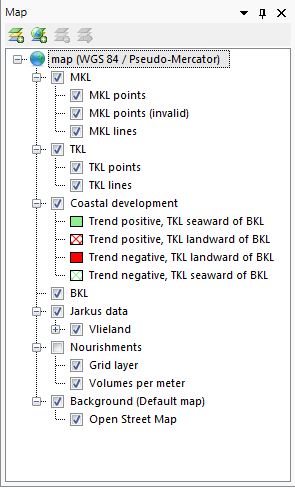
\includegraphics{figures/chapter_general/Map_Contents.png}
		\caption{Voorbeeld van het Map toolvenster waarin verschillende kaartlagen worden getoond. In dit geval gaat het om de kaartlagen van het resultaat van een Momentary coastline model.}
	\label{fig:Map_Contents}
\end{figure}

Door op een laag rechts te klikken wordt een menu geopend dat de mogelijkheden weergeeft voor die laag (figuur \ref{fig:MapLayer_Context_Menu}). Hieronder vallen bijvoorbeeld:
\begin{itemize}
\item \textbf{Properties} - bewerk de styling van de laag. Hiermee kunnen de kleur(schaal) en weergave van de features op deze laag worden aangepast. Tevens is dit de plaats om labels aan of uit te zetten.
\item \textbf{Zoom to Extent} - zet het zoom niveau van de kaart dusdanig dat alle informatie van deze laag precies in het beeld past
\item \textbf{Show in legend} - laat deze laag in de legenda van de kaart zien
\item \textbf{Hide all layers but this one} - laat alleen deze laag op de kaart zien en zet de anderen uit
\end{itemize}

\begin{figure}[h!]
	\centering
		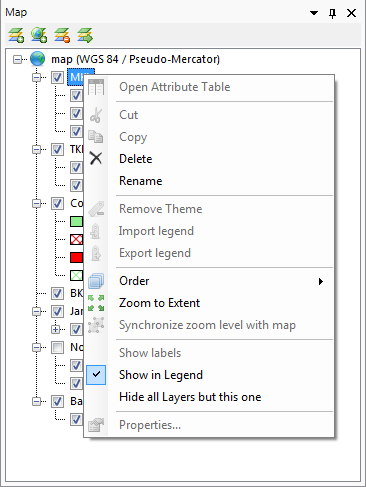
\includegraphics{figures/chapter_general/rt_MapLayer_Context_Menu.png}
		\caption{menu met mogelijkheden na het rechts klikken op een kaartlaag}
	\label{fig:MapLayer_Context_Menu}
\end{figure}

\subsection{Chart toolvenster}
	\label{RT_Chart_Contents}
Indien een document venster een grafiek bevat laat het \textbf{Chart} toolvenster (figuur \ref{fig:3_Chart_Contents}) de afzonderlijk getekende lijnen en punten met hun eigenschappen zien. Door op een item in het toolvenster te klikken (selecteren) wordt in het \textbf{Properties} toolvenster de eigenschappen getoond. Deze kunnen worden bewerkt, zodat bijvoorbeeld het bereik van de assen kan worden veranderd, of kleuren en namen kunnen worden aangepast. Hierdoor is het mogelijk om de figuren met vaste assen te exporteren. Ook kunnen bepaalde lijnen of punten tijdelijk aan of uitgezet worden. In de huidige versie van RT is deze functie helaas nog niet voor de transect editor beschikbaar.

\begin{figure}[H]
	\centering
		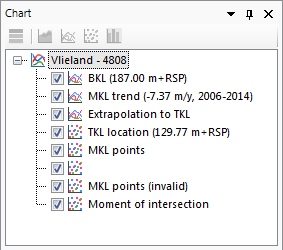
\includegraphics{figures/chapter_general/Chart_Contents.png}
		\caption{Voorbeeld weergave van het Chart toolvenster}
	\label{fig:3_Chart_Contents}
\end{figure}

\subsection{Properties}
Wanneer een element in de interface is geselecteerd (bijvoorbeeld in het project toolvenster, op een kaart, een resultaat grafiek of in het chart tool venster) worden de eigenschappen van dit element weergegeven in het \textit{Properties} toolvenster. Naast het geven van een overzicht van de eigenschappen van een geselecteerd element, wordt het \textit{Properties} venster ook gebruikt voor het bewerken van de getoonde eigenschappen.
De eigenschappen kunnen gegroepeerd worden, of alfabetisch gesorteerd worden.
Onder aan het \textit{Properties} toolvenster wordt er een uitgebreide beschrijving van het geselecteerde veld in het \textit{Properties} toolvenster.

\subsection{Time Navigator}
	\label{sec:TimeSeriesNavigator}
De time navigator wordt gebruikt om te navigeren door tijd(stappen) van een tijdsafhankelijke variabele. Elk scherm dat tijdsafhankelijke informatie toont heeft zijn eigen time navigator. Hiermee is er de mogelijkheid om te navigeren door de tijd. Deze tijdnavigatie kan twee vormen aannemen:
\begin{itemize}
\item Enkele tijdsindicatie. In dit geval heeft de tijdnavigatie balk een verticale lijn die de positie in de tijd aangeeft. In dit geval wordt slechts een tijdstip weergegeven en wel het tijdstip links van de genoemde lijn (zie \Fref{fig:TimeSeriesNavigator}). 
\item Tijd range (figuur \ref{fig:TimeSeriesNavigator_Range}). In dit geval heeft de navigatie balk een rechthoek die begin en eind tijdstip aangeeft. In dit geval worden alle gegevens tussen het begin en eind tijdstip weergegeven.
\end{itemize}

\begin{figure}[H]
	\centering
		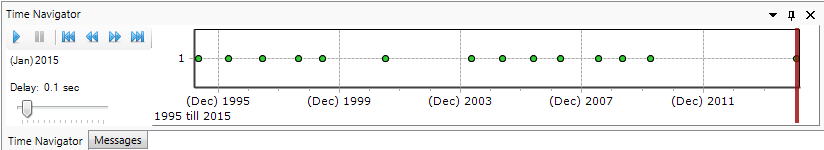
\includegraphics[width=\textwidth]{figures/chapter_general/TimeSeriesNavigator.png}
		\caption{Time Navigator met enkele tijdsindicatie}
	\label{fig:TimeSeriesNavigator}
\end{figure}

\begin{figure}[H]
	\centering
		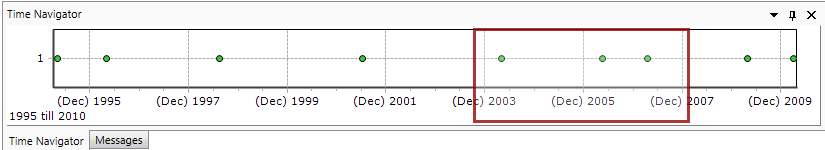
\includegraphics[width=\textwidth]{figures/chapter_general/TimeSeriesNavigator_Range.png}
		\caption{Time Navigator met tijdrange weergave}
	\label{fig:TimeSeriesNavigator_Range}
\end{figure}

\subsection{Messages}
	\label{sec:RT_Messages}
Het \textit{Messages } venster is een loggingvenster. Berichten verstuurd uit modellen of verschillende delen van het systeem worden hier chronologisch getoond (hoe verder naar beneden, des te ouder het bericht). De informatie van elk bericht wordt getoond in drie kolommen (zie \Fref{fig:general.messagesPanel}). Afhankelijk van de inhoud van het bericht worden deze weergegeven met een icoon in de eerste kolom (zie voor een verklaring van de iconen tabel \ref{table:message_icons}). De tweede kolom geeft weer de tijdstip waarop het bericht gegenereerd werd. Op de derde kolom, wordt de tekst met de informatie van het bericht weergegeven.

\begin{table}[H]
\caption{Bericht types}
\centering
\begin{tabular}{| c | l |}
\hline
\STRUT{\bf Icoon} & {\bf Bericht type}\\ [1ex]
\hline
\rule{0in}{4ex} 
\includegraphics{figures/chapter_general/Message_Icon_Info.png} & Informatie \\
\hline
\rule{0in}{4ex}

\includegraphics{figures/chapter_general/Message_Icon_Warning.png} & Waarschuwing \\
\hline
\rule{0in}{4ex}

\includegraphics{figures/chapter_general/Message_Icon_Error.png} & Error \\
\hline
\end{tabular}
\label{table:message_icons}
\end{table}

Door de drie meest linkse icoontjes boven aan de berichtenlijst aan al dan uit te zetten, kan er vastgelegd worden welke types van berichten in het \textit{Messages} venster getoond worden. Deze knoppen kunnen op elk moment bediend worden, en deze actie veroorzaakt niet dat er berichten gewist worden. Deze icoontjes controleren alleen maar de zichtbaarheid van de verschillende berichttypes. 

Het meest rechtse icoontje wordt gebruikt om het laatst geselecteerde bericht in een apart venster te laten zien. Dit is handig als de tekst van het bericht lang is, om hem beter te kunnen bestuderen en, eventueel, deels of volledig kopi\"{e}ren naar het klembord.

\begin{figure}[H]
	\centering
		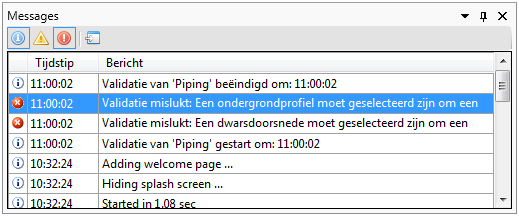
\includegraphics{figures/chapter_general/messagesPanel}
		\caption{Time Navigator met tijdrange weergave}
	\label{fig:general.messagesPanel}
\end{figure}

Het is mogelijk om alle berichten van alle types in een klap te wissen. Dit kan door de optie \textit{Verwijder alles} te kiezen in het context menu op het loggingvenster (\Fref{fig:general.messagesPanelContextMenu}). Indien het venster wordt gesloten en weer geopend (zie paragraaf \ref{sec:RT_Docking}) worden ook alle eerdere berichten gewist en alleen de nieuwe berichten worden eraan bijgevoegd. In hetzelfde contextmenu (\Fref{fig:general.messagesPanelContextMenu}) bestaat er ook een optie om alle geselecteerde regels naar het klembord te kopi\"{e}ren.

\begin{figure}[H]
	\centering
		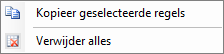
\includegraphics{figures/chapter_general/messagesPanelContextMenu}
		\caption{Time Navigator met tijdrange weergave}
	\label{fig:general.messagesPanelContextMenu}
\end{figure}

Hiernaast, wordt een applicatie log bijgehouden voor elke sessie (van opstarten tot afsluiten) van Ringtoets in de project database. In deze log-file worden alle berichten opgeslagen die zich tijdens de sessie voordoen. De applicatie log kan ten alle tijden worden opgevraagd door (zie \Fref{fig:general.openLog}) te klikken op \textbf{File} $\rightarrow$ \textbf{Help} $\rightarrow$  \textbf{Show Log}.

\begin{figure}[H]
	\centering
		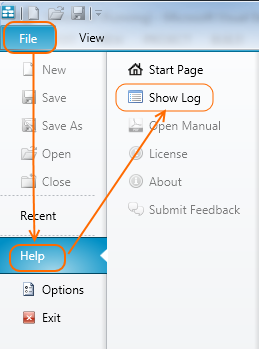
\includegraphics{figures/chapter_general/openLog}
		\caption{Log van Ringtoets openen.}
	\label{fig:general.openLog}
\end{figure}



\section {Import \ Export}
Indien voor een item in het \textbf{Project} toolvenster een zogenaamde exporter of importer is gedefinieerd, is het in RT mogelijk om gegevens te exporteren of importeren via het menu onder de rechter muisknop. Kies hiervoor \textbf{Export...} of \textbf{Import...}. Indien een plugin of het framework zelf een exporter of importer voor het geklikte item is aangeboden kan deze worden gebuikt. In sommige gevallen zijn er meerdere manieren om items te exporteren (bijvoorbeeld berekeningsresultaten kunnen als figuur worden ge"exporteerd, maar ook naar het csv format dat in Excel leesbaar is).

RT definieert voor alle berekeningsresultaten een exporter die de resultaten wegschrijft als csv file. Dit format is eenvoudig in Microsoft Excel in te lezen. Let er op dat als scheidingsteken voor de verschillende cellen een "';"' wordt gebruikt en dat in alle gevallen een "'."'  de scheiding tussen gehele getallen en de decimalen aangeeft.